% Created 2015-04-02 Thu 14:20
\documentclass[11pt]{article}
\usepackage[utf8]{inputenc}
\usepackage[T1]{fontenc}
\usepackage{fixltx2e}
\usepackage{graphicx}
\usepackage{longtable}
\usepackage{float}
\usepackage{wrapfig}
\usepackage{soul}
\usepackage{textcomp}
\usepackage{marvosym}
\usepackage{wasysym}
\usepackage{latexsym}
\usepackage{amssymb}
\usepackage{hyperref}
\tolerance=1000
\usepackage{methodshw, amsmath}
\providecommand{\alert}[1]{\textbf{#1}}

\title{8004 Homework 8}
\author{Nooreen Dabbish}
\date{\today}
\hypersetup{
  pdfkeywords={},
  pdfsubject={},
  pdfcreator={Emacs Org-mode version 7.9.3f}}

\begin{document}

\maketitle




\section{This is Problem 3 of Faraway (2006), Chapter 9}
\label{sec-1}


The \verb~ratdrink~ data consist of five weekly measurements of body
weight for 27 rats. The first 10 rats are on a control treatment
while seven rats have thyroxine added to their drinking water. Ten
rats have thiouracil added to their water. Build a model for the rat
weights that shows the effect of the treatment.


\begin{verbatim}
library(faraway)
data(ratdrink)
\end{verbatim}
\subsection{Model the weights of the rate, incorporating the treatment effects and random effect. Use \verb~R~ to fit the model.}
\label{sec-1-1}


We write y$_{\mathrm{ijk}}$ to represent the kth rat in the jth treatment group
on the ith week, where (i=1,2,3,4), (j=1,2,3), and (k= 1-10 for
control, k = 1-7 thyroxine, and k = 1-10 for thiouracil). $\mu$
represents the overall mean weight, $\alpha$$_i$ represents the fixed
effect contribution of the ith week, $\beta$$_j$ repsents the fixed
effect contribution of the jth treatment, and $\delta$$_{\mathrm{ij}}$ is the
interaction of weeks and treatment. The random effect u$_{\mathrm{jk}}$
incorporates the repeated measures of the same rat.

$$y_{ijk} = \mu + \alpha_i + \beta_j + \delta_{ij} + u_{jk} + \epsilon_{ijk}$$




To fit the model in R we write:


\begin{verbatim}
library(lme4)
rat.lme <- lmer(wt ~ weeks+ treat+ weeks*treat+ (1|subject))
summary(rat.lme)
\end{verbatim}
\subsection{What is the implication of the random effect on the correlations between weights of the same rat? Is that implication reasonable? It would be nice to support your argument with data evidence.}
\label{sec-1-2}


The random effect captures the fact that weights measured from the
same rat are correlated whereas weights from different rats are
uncorrelated. This is reasonable because even if a treatment makes
rats A and B lose weight at the same rate, say x grams/week, they
will weight A-x and B-x respectively.
\section{The article “Variability of Sliver Weights at Different Carding Stages and a Suggested Sampling Plan for Jute Processing”}
\label{sec-2}

by A. Lahiri (Journal of the Textile Institute, 1990) concerns the 
partitioning
of variability in “sliver weight.” (A sliver is a continuous strand
of loose, untwisted wool, cotton,
etc., produced along the way to making yarn.) For a particular mill, 
3 (of many) machines were
studied, using 5 (10 mm) pieces of sliver cut from each of 5 rolls produced on the machines. The
weights of the (75) pieces of sliver were determined and a standard hierarchical (balanced data)
ANOVA table was produced as below. (The units of weight were not given in the original article.)


\begin{center}
\begin{tabular}{lrr}
 Source    &    SS  &  df  \\
\hline
 Machines  &  1966  &   2  \\
 Rolls     &   644  &  12  \\
 Pieces    &   280  &  60  \\
\hline
 Total     &  2890  &  74  \\
\end{tabular}
\end{center}




The model is $$y_{ijk} = \mu + \alpha_i +u_{ij} + \epsilon_{ijk}$$

for the kth piece of the jth roll on the ith machine, where
$\alpha_i \overset{iid}{\sim} N(0,\sigma^2_\alpha)$,
$\u_{ij} \overset{iid}{\sim} N(0,\sigma^2_u)$, and $\epsilon_i \overset{iid}{\sim} N(0,\sigma^2_\epsilon)$,  
\section{Appendix: Tangled R Code}
\label{sec-3}


\lstinputlisting{DabbishHW8.R} 
\section{Appendix: Initial evaluation of ratdrink dataset}
\label{sec-4}


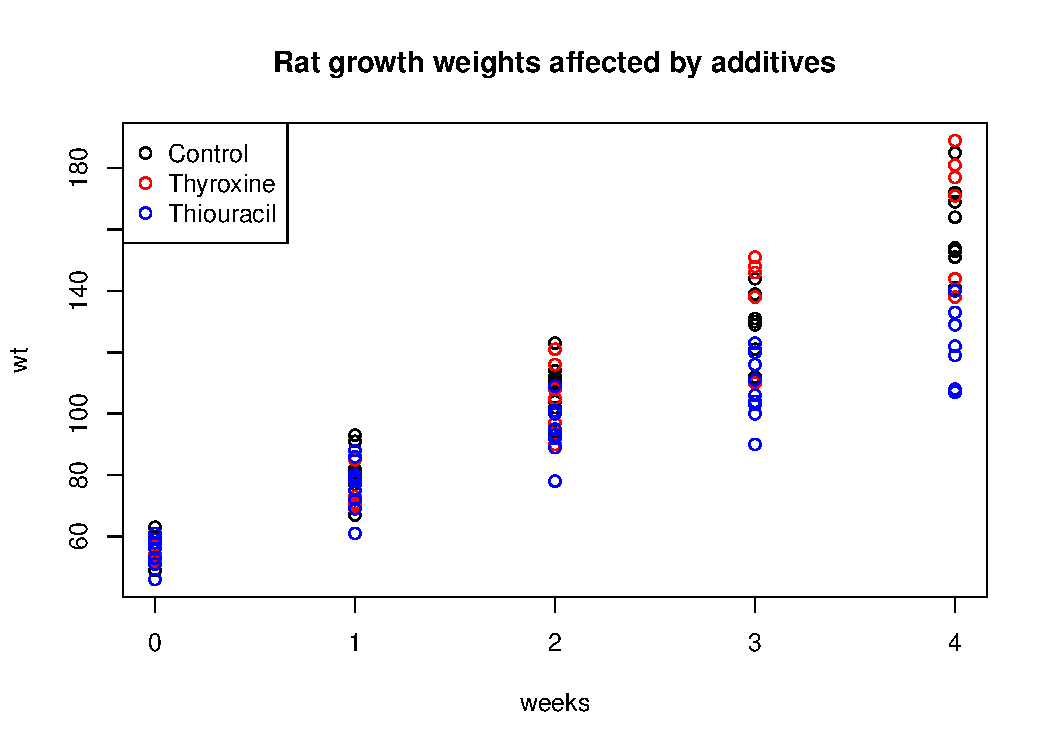
\includegraphics[width=.9\linewidth]{./ratweights.pdf}

Plotting the ratdrink data suggested that rats that drank Thyroxine
tended to have increased body weight after 5 weeks in comparison to rats
drinking Thiouracil and Control. The rats that drank Thiouracil
tended to have lowerbody weight than the Control and Thyroxine groups.

\end{document}
